 \documentclass{standalone}
  \usepackage{subfigure} 
  \usepackage{graphicx}
 
 \begin{document}
 	\begin{figure}
    	\centering
		\subfigure[][]{
			\label{fig:ex3-a}
			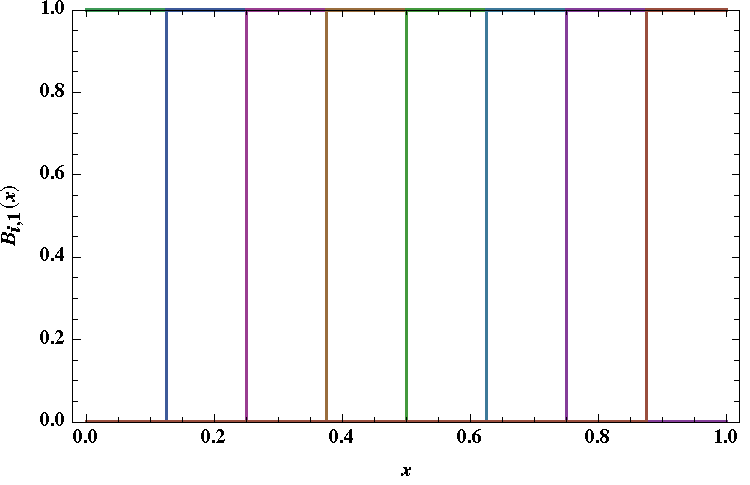
\includegraphics[height=2in]{Bsp1.pdf}}
		\hspace{8pt}
		\subfigure[][]{
			\label{fig:ex3-b}
			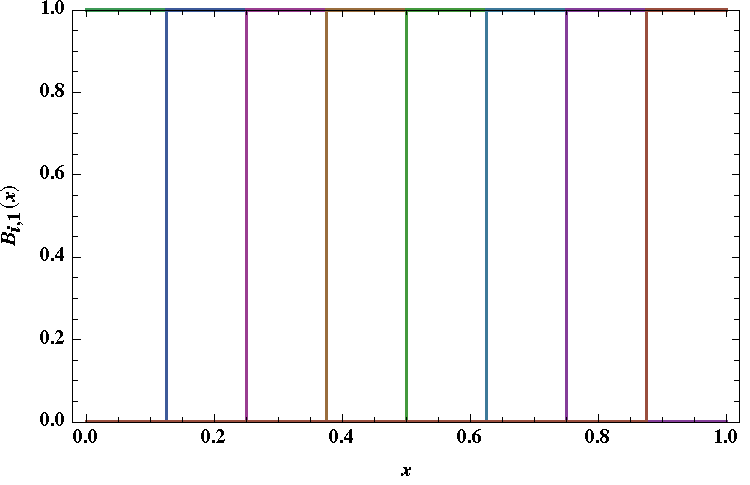
\includegraphics[height=2in]{Bsp1.pdf}} \\
		\subfigure[][]{
			\label{fig:ex3-c}%
			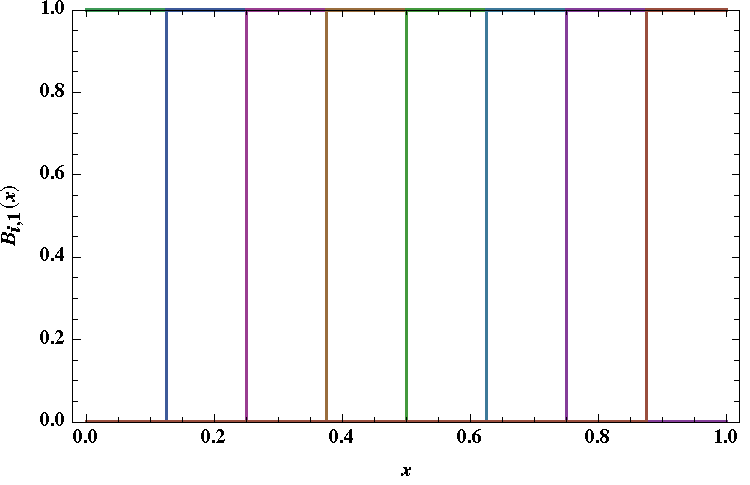
\includegraphics[height=2in]{Bsp1.pdf}}
		\hspace{8pt}
		\subfigure[][]{
			\label{fig:ex3-d}
			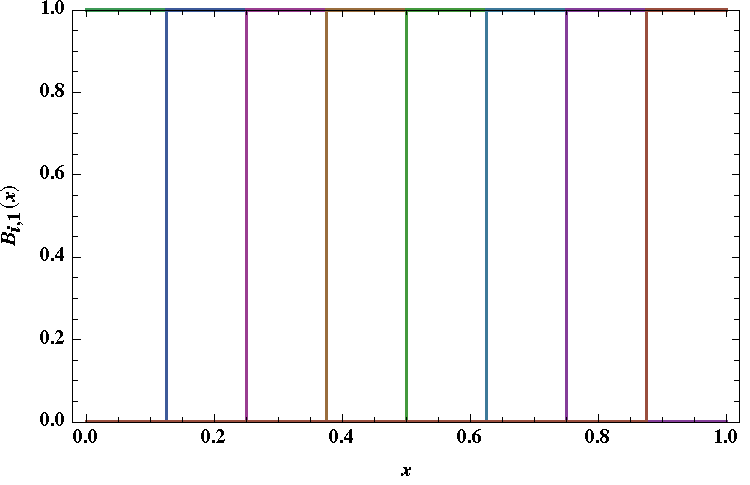
\includegraphics[height=2in]{Bsp1.pdf}}
		\caption[A set of four subfigures.]{A set of four subfigures:
			\subref{fig:ex3-a} describes the first subfigure;
			\subref{fig:ex3-b} describes the second subfigure;
			\subref{fig:ex3-c} describes the third subfigure; and,
			\subref{fig:ex3-d} describes the last subfigure.}
		\label{fig:ex3}
	\end{figure}
\end{document}